\section{Stage}

\subsection{Analisi dei requisiti}
L'azienda in cui ho svolto l'attività di stage universitario opera
principalmente nel settore assicurativo producendo gestionali per
semplificare l'amministrazione degli utenti, delle scadenze delle polizze,
degli avvisi di pagamento, della rateizzazione... \\
In particolare si cerca di semplificare tutto il procedimento che viene svolto
dai vari broker assicurativi durante il procedimento di ricerca e stipula di
una polizza, dalla realizzazione di preventivi basati sulle richieste
specifiche del cliente fino alla stipula del contratto.
Tra le varie funzionalità che offrono i loro prodotti c'è anche la possibilità
di salvare i documenti dei clienti, in particolare i contratti firmati 
direttamente all'interno del programma, Ovviamente questi documenti sono
salvati in modo sicuro e protetto da accessi non autorizzati e per essi deve 
essere garantita l'integrità e l'autenticità. \\
La tecnica che viene utilizzata per garantire l'integrità è quella
dell'hashing, in particolare viene calcolato l'hash di alcuni meta-dati del
file e viene poi salvato all'interno del database, in questo modo è possibile
verificare che il file non sia stato modificato in alcun modo e sia quindi
integro. \\
Per quanto riguarda l'autenticità invece viene utilizzata una firma digitale
che viene apposta sul file, in questo modo è possibile verificare che il file
sia stato firmato da una persona autorizzata e che quindi sia autentico. 

\subsubsection{Problemi da risolvere}
Il sistema utilizzato dall'azienda è abbastanza solido e viene utilizzato da
anni, tuttavia si è cercato un modo per migliorarlo e renderlo più sicuro e
affidabile. \\
Tra le varie problematiche che sono emerse c'è quella relativa al salvataggio
dell'hash-code all'interno del database, in particolare se un utente
malintenzionato riuscisse ad accedere al database potrebbe modificare
l'hash-code e quindi invalidare il file. Inoltre se l'utente riuscisse ad
accedere al file potrebbe modificarlo e poi aggiornare l'hash-code nel database
in modo da rendere il file integro. \\
Serviva trovare un modo per garantire in modo trasparente al cliente che
l'hash-code salvato non potesse essere in nessun modo modificato.

\subsubsection{Soluzioni proposte}
Sono state proposte varie soluzioni tra cui quella di salvare in molteplici
database l'hash-code in modo da rendere più difficile la modifica, oppure
quella di salvare l'hash-code in un database esterno ad esempio online,
ma tutte queste soluzioni non risolvevano il problema di base, ovvero che
l'hash-code poteva essere modificato. \\
Infatti queste proposte non andavano a cambiare l'idea di fondo, ossia 
l'utilizzo di un database per salvare il codice, ma cercavano solamente 
di aumentare il coefficiente di difficoltà per un utente malintenzionato,
ma si portavano dietro tutti i problemi che c'erano prima.
Quindi dopo varie discussioni è stata avanzata l'idea di utilizzare la
tecnologia blockchain per risolvere il problema.

\newpage

\subsection{Soluzione: Blockchain}
\subsubsection{Introduzione}
La blockchain è una tecnologia che permette di salvare dati in modo sicuro e
affidabile, in particolare i dati vengono salvati in blocchi che vengono poi
concatenati tra loro in modo da formare una catena, da qui il nome
blockchain.\\
L'integrità dei dati è garantita dal fatto che ogni blocco contiene l'hash-code
del blocco precedente, in questo modo se un utente malintenzionato volesse
modificare un blocco dovrebbe modificare anche tutti i blocchi successivi,
rendendo praticamente impossibile la modifica.
Inoltre i blocchi vengono salvati in modo distribuito, in questo modo non c'è
un unico punto di accesso ai dati, ma sono distribuiti in modo che tutti gli
utenti possano accedervi. Ogni utente ha una copia della blockchain e può
verificare che i dati siano corretti e che non siano stati modificati e questo
garantisce la trasparenza del sistema.

\subsubsection{Quali dati salvare}
La blockchain è una tecnologia molto potente e versatile, ma non è adatta a
qualsiasi tipo di dato, infatti è stata progettata per salvare transazioni
di denaro e non per salvare file. \\
Quindi, l'opzione di salvare l'intero documento all'interno della blockchain
è stata scartata, in quanto sarebbe stato troppo dispendioso in termini di
risorse e non sarebbe stato possibile salvare grandi moli di dati. Inoltre 
sarebbe stato anche uno spreco di risorse dato che i documenti vengono già
salvati in modo sicuro all'interno del database dei clienti. \\
Quindi si è deciso di salvare solamente l'hash-code del documento all'interno
della blockchain in modo da ridurre l'utilizzo di risorse e allo stesso tempo
garantire l'integrità del file.
Quindi il processo utilizzato in precedenza viene preservato, ma serviva 
solamente cambiare il modo in cui viene salvato il codice di verifica.

\subsubsection{Come interagire con la blockchain}
La tecnologia della blockchain è sembrata fin da subito una buona soluzione, 
ora serviva trovare un modo per integrarla con il sistema già esistente in 
modo da non alterare l'utilizzo del programma da parte degli utenti finali.
Per implementare l'invio dei dati lato applicazione bastava creare un nuovo
processo come quelli che erano già presenti che periodicamente inviasse i 
nuovi dati. Quindi alla fine si trattava solamente di adattare il codice 
già esistente che salvava sul database.
Tuttavia serviva capire come creare un punto d'accesso dal lato blockchain
a cui poter inviare le richieste.

\subsubsection{Smart Contract}
Alcune blockchain come Ethereum permettono di creare degli smart contracts,
ovvero dei programmi che vengono eseguiti all'interno della blockchain e che
possono interagire con essa. \\
In realtà gli smart contracts non sono dei veri e propri programmi in quanto
non possono interagire con l'input dell'utente, non possono fare delle chiamate
http e non possono accedere a risorse esterne, ma possono solamente eseguire
una lista di operazioni descritta dal programmatore. In sostanza sono delle
macchine a stati finiti che vengono eseguite all'interno della blockchain e con
la quale possono interagire direttamente. \\
La caratteristica di questa tecnologia è che gli smart contracts sono dei 
contratti senza intermediari che vengono eseguiti in modo automatico e senza 
nessun supervisore umano, quindi potenzialmente potrebbero essere utilizzate
per stipulare, ad esempio, delle polizze assicurative totalmente gestite
da sistemi informatici. Nel nostro caso bastava questa caratteristica non è
stata necessaria in quanto dovevamo solo salvare dei dati.
Le interfacce che sono state create sono le seguenti:
\begin{itemize}
    \item \textbf{saveHashCode(...)}: per inserire un nuovo hash-code
        all'interno della blockchain. 
    \item \textbf{getHashCode(...)}: per ottenere l'hash-code di un file.
\end{itemize}

\newpage

\subsection{Struttura del progetto}
Il gestionale su cui ho dovuto lavorare si divideva principalmente in due parti
logiche separate:
\begin{itemize}
    \item \textbf{Parte grafica e funzionale}: è la parte che comprende il
        front-end e il back-end, si occupa di fornire l'interfaccia grafica
        all'utente e di gestire le richieste che arrivano dal client.
    \item \textbf{Parte dei processi}: è la parte che si occupa di eseguire
        periodicamente una serie di processi, principalmente di invio notifiche 
        o di sincronizzazione dei dati.
\end{itemize}
Il mio compito è stato quello di modificare la parte dei processi in modo da
aggiungere il processo che si occupa di inviare i dati alla blockchain. \\
Il resto del codice non aveva bisogno di essere modificato in quanto il tutto
era già utilizzato per mandare i documenti e gli hash-code al database, quindi
abbiamo solo dovuto modificare il processo che salva il codice di verifica.

\subsubsection{Analisi struttura del codice}
Dovendo lavorare solo sulla parte dei processi, ho dovuto analizzare il codice
per capire come funzionava e come potevo integrare la blockchain. \\
Il progetto sostanzialmente contiene una serie di classi che contengono la
logica che deve essere eseguita dal processo e poi una libreria che si occupa
della configurazione e dell'esecuzione dei processi. \\
Ovviamente il progetto contiene anche delle utility per poter interagire
tramite chiamate http e per poter eseguire operazioni sul database.
\begin{figure}[H]
    \centering
    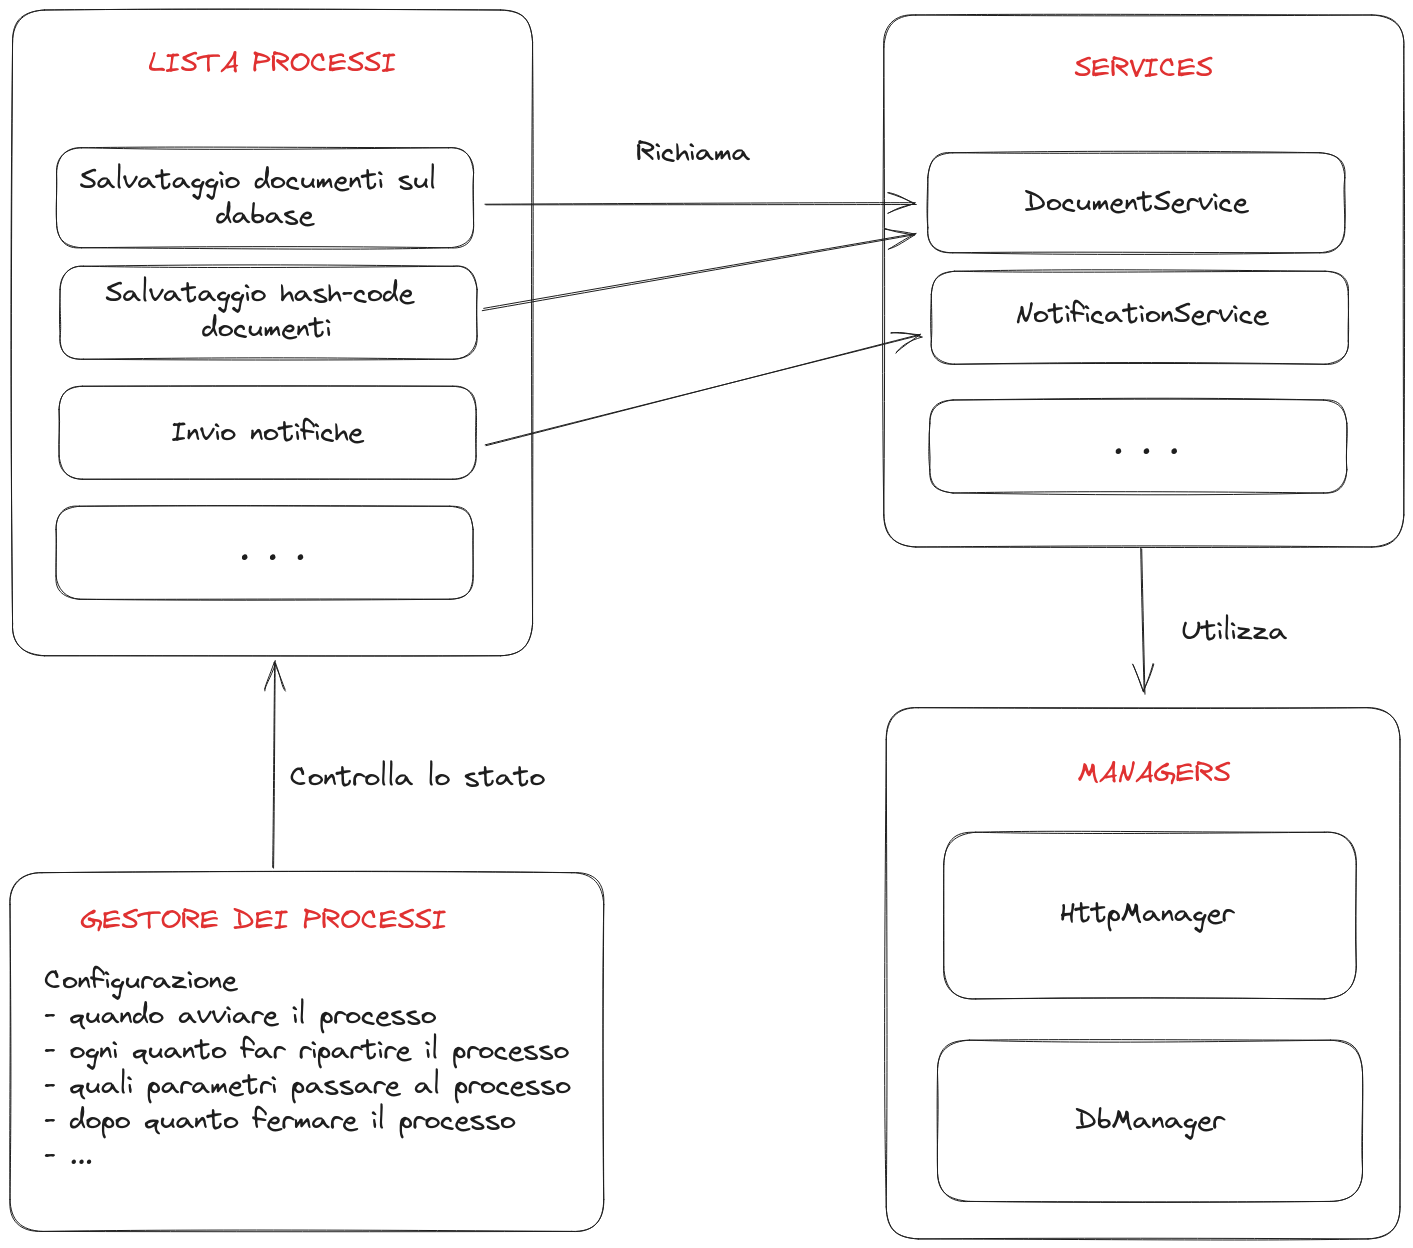
\includegraphics[width=0.9\textwidth]{ProcessManagerProjectComponents.png}
    \caption{Struttura del progetto di gestione dei processi}
    \label{fig:process-manager-project-components}
\end{figure}

Come si può vedere dalla figura \ref{fig:process-manager-project-components} il
progetto ha quattro parti fondamentali:
\begin{itemize}
    \item \textbf{Gestore dei processi}: è la libreria che si occupa di gestire
        i processi, in particolare si occupa di leggere la configurazione e di
        eseguire i processi. La configurazione è un file json che contiene
        informazioni riguardo al nome del processo, i dati da passare, quando
        eseguire e ogni quanto riavviare il processo ...
    \item \textbf{Processi}: sono le classi che contengono la logica che deve
        essere eseguita dal processo, in particolare ogni classe deve
        implementare l'interfaccia \textit{IProcess} che contiene il metodo
        \textit{execute()} che viene eseguito dal gestore dei processi. Il
        processo non contiene effettivamente il codice che implementa le
        funzioni che devono essere eseguite, ma richiama le interfacce fornite
        dal Service di riferimento. 
    \item \textbf{Services}: sono le classi che vengono richiamate dal processo
        e che contengono le interfacce di comunicazione tra il processo e il
        manager. Queste classi esistono per nascondere le implementazioni del
        manager e per racchiudere più istruzioni in un unica chiamata. Per
        esempio un interfaccia può gestire l'intero salvataggio del documento,
        ma al suo interno richiama due funzioni del manager, una per il
        salvataggio dei dati del documento e una per il salvataggio
        dell'hash-code
    \item \textbf{Magagers}: sono le classi che si occupano di interagire
        direttamente con dei servizi tramite chiamate http, o di eseguire
        operazioni sul database, oppure di comunicare con altri servizi.
\end{itemize}

\subsubsection{Analisi funzionamento dei processi}
La maggior parte dei processi implementati dal software funzionano tramite la
logica di una coda di richieste (FIFO).

\begin{figure}[H]
    \centering
    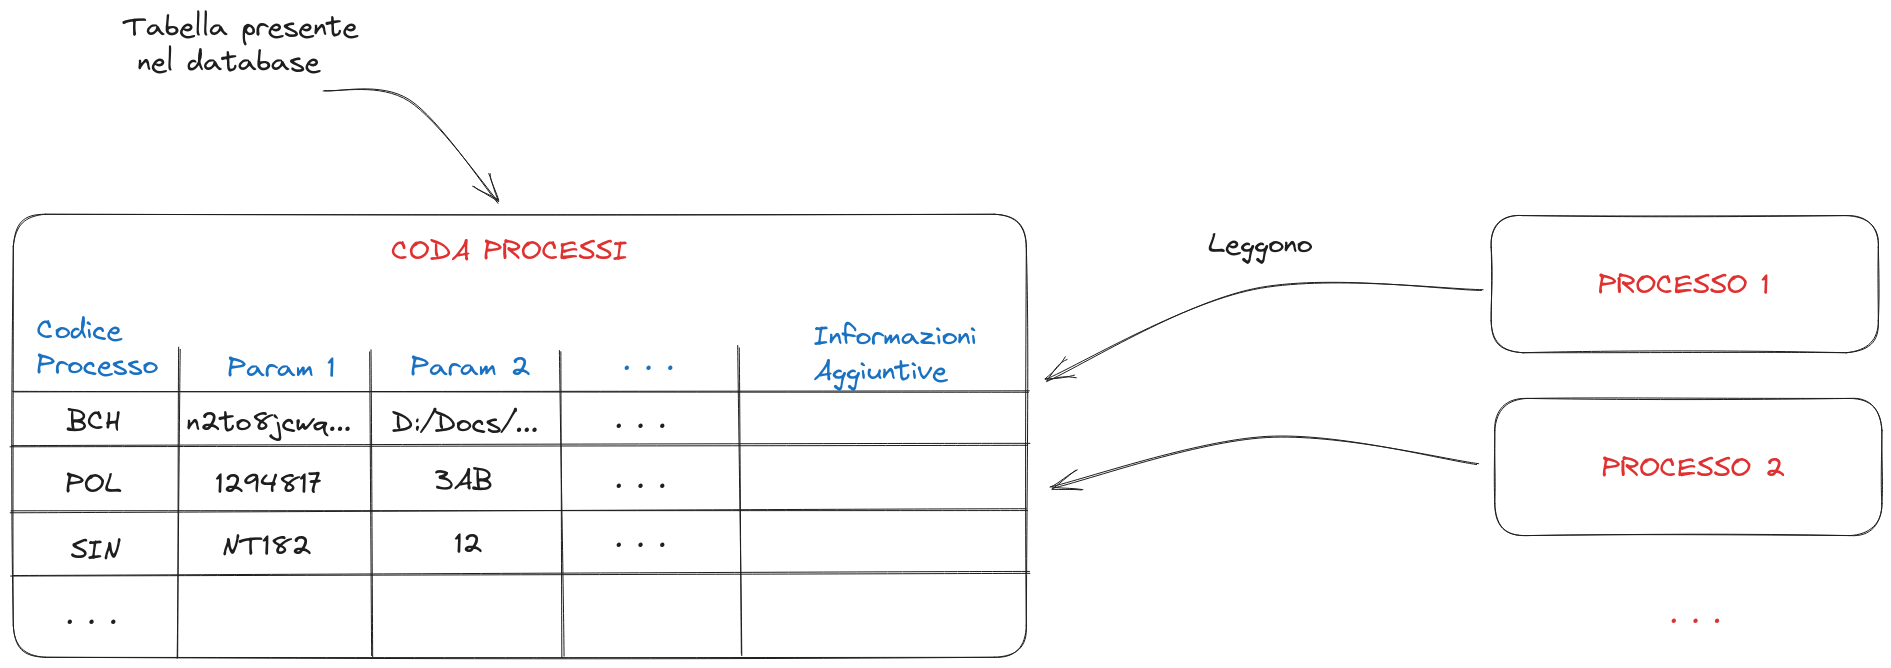
\includegraphics[width=0.9\textwidth]{DatabaseProcessTableSchema.png} 
    \caption{Tabella contenente la lista dei processi}
    \label{fig:table-process-list}
\end{figure}

La figura \ref{fig:table-process-list} mostra lo schema di funzionamento della 
coda dei processi. \\
Sostanzialmente esiste una tabella nel database che su ogni record contiene
dei dati che possono essere letti ed interpretati dai singoli processi e che 
ne determinano il funzionamento. \\ 
Ogni record contiene una serie di dati obbligatori e altri dati che invece 
sono opzionali. I dati obbligatori sono:
\begin{itemize}
    \item \textbf{Codice Processo}: è un codice che identifica il processo che
        deve essere eseguito. Questo codice viene utilizzato per capire quale
        classe deve essere eseguita dal gestore dei processi. Viene scelto 
        arbitrariamente dal programmatore e salvato in un file di 
        configurazione all'interno del codice del programma.
    \item \textbf{Parametri}: una serie di colonne che sono adibite al passaggio
        di parametri al processo. Questi parametri possono essere utilizzati 
        per passare dati che sono necessari al processo per poter funzionare.
        Un esempio di parametro può essere il nome del file che deve essere
        salvato o il nome della cartella in cui deve essere salvato.
    \item \textbf{Dati utente}: una serie di dati che identificano l'utente che
        ha richiesto l'esecuzione del processo. Questi dati sono utili
        in caso di problemi o di errori, in modo da poter risalire all'utente
        che ha fatto partire la richiesta e poterlo contattare.
    \item \textbf{Dati aggiuntivi}: sono dati che come quelli dell'utente
        servono in caso di problemi. Possono essere dati aggiuntivi le 
        informazioni riguardo alla data di inserimento e di esecuzione del 
        processo, il nome della macchina che ha aggiunto e quella che ha 
        eseguito il processo ...
\end{itemize}

La tabella viene popolata automaticamente da altri processi oppure vengono
inseriti nuovi record in base alle operazioni eseguite dall'utente. Per esempio
se un utente richiede il salvataggio di un nuovo documento tramite
l'interfaccia grafica, allora viene inserito dal programma una nuova richiesta
nella tabella con i dati necessari a far funzionare il processo di
conservazione.

\subsection{Implementazione}
Per sviluppare questo progetto ho dovuto per prima cosa creare un mio processo
e il relativo codice-processo nel file di configurazione. Al processo è stato
assegnato il codice BCH (che identifica il salvataggio su blockchain) e il
processo è stato chiamato \textit{BlockchainConservationProcess}. \\
Il processo non ha nulla di particolare al suo interno, semplicemente va a 
leggere i dati dal database e quando trova nella coda dei processi il suo codice
allora estrae i parametri dal record sul database e richiama le funzioni per 
eseguire il salvataggio su blockchain. \\
Al processo vengono passati i seguenti valori:
\begin{itemize}
    \item \textbf{Hash-Code}: il codice viene generato da un algoritmo già 
        utilizzato all'interno del programma che estrae alcuni dati dalle 
        informazioni del documento e ne genera un codice univoco.
    \item \textbf{Codici aggiuntivi}: una serie di parametri aggiuntivi che
        servono sempre all'interno della logica del gestionale, ma che per me
        non hanno nessun importanza in quanto non vengono utilizzati, è solo
        importante salvarli in modo sicuro.
\end{itemize}

Ora che il processo è stato creato, ho dovuto creare il codice che si occupa
di interagire con la blockchain, il punto focale di questo progetto. \\
Per poterlo realizzare ho utilizzato la tecnologia degli smart-contract che ho
sviluppato tramite il linguaggio Solidity. 

Solidity è un linguaggio di programmazione ad alto livello utilizzato per
scrivere smart contract sulla blockchain Ethereum. Grazie a Solidity, gli
sviluppatori possono creare applicazioni decentralizzate (DApps) sulla
blockchain Ethereum, che possono essere utilizzate per una vasta gamma di
scopi, come ad esempio la gestione di token, la registrazione di proprietà
intellettuale, la gestione dei contratti e molto altro ancora.

Per poter scrivere codice Solidity ho utilizzato l'editor di testo Remix, 
un editor online che permette di testare i propri smart-contract su delle 
blockchain di test, in modo da non aver nessun costo di transazione.
Infatti un fattore da considerare è che ogni transazione che viene eseguita
sulla blockchain ha un costo, che viene pagato in Ether, la valuta della
blockchain Ethereum. Anche il deploy di uno smart-contract è una transazione
e perciò ha un costo. Per questo motivo esistono delle blockchain di test,
realizzate appositamente per permettere agli sviluppatori di testare i propri
codici senza dover ogni volta pagare. L'IDE online Remix aiuta proprio a fare
questo, permettendo di scegliere in modo facile su quale blockchain salvare
il proprio smart-contract. Questo ovviamente sarebbe stato possibile anche
senza Remix, ad esempio scaricando dei software che eseguono
una blockchain di test sulla propria macchina come ganache-cli, ma l'IDE
online è molto più comodo e veloce da utilizzare. \\
Inoltre Remix ha una grafica che offre un'interfaccia che aiuta anche a 
visualizzare i costi effettivi del deploy e delle transazioni, oltre ad avere
già installate tutte le versioni del compilatore e del debugger, in modo 
da poterli cambiare velocemente e senza doverli scaricare.

\newpage

Il codice Solidity è contenuto in un file con estensione \textit{.sol} ed
è composto come segue:
\begin{lstlisting}[language=Solidity]
// SPDX-License-Identifier: MIT
pragma solidity ^0.8.0;
contract MyContract {
    function helloWorld() public pure returns (string memory) {
        return "Hello, World!";
    }
}
\end{lstlisting}
In questo esempio si possono vedere alcune parti fondamentali del codice:

\begin{itemize}
    \item \textbf{Versione di Solidity}: con il codice \textit{pragma solidity
        \^0.8.0} si indica la versione del compilatore di Solidity che deve
        essere utilizzata per compilare il codice. Questo è importante in
        quanto ogni versione del compilatore ha delle caratteristiche diverse
        e quindi è importante specificare la versione che si vuole utilizzare.
    \item \textbf{Contratto}: con la parola chiave \textit{contract} si indica
        che si sta definendo un nuovo contratto. Il contratto è l'oggetto
        principale di Solidity, è l'oggetto che viene salvato sulla blockchain
        e che contiene tutte le funzioni e le variabili che si vogliono
        utilizzare. Il nome del contratto è il nome inserito dopo la keyword
        \textit{contract}, in questo caso \textit{MyContract}.
    \item \textbf{Funzioni}: Le funzioni in Solidity sono come le funzioni in
        altri linguaggi di programmazione, ma hanno alcune caratteristiche
        particolari. Per prima cosa le funzioni possono avere due livelli di
        visibilità: public o internal. Le funzioni pubbliche possono essere
        chiamate da chiunque, mentre le funzioni internal possono essere
        chiamate solo da altre funzioni all'interno del contratto. Inoltre le
        funzioni possono avere delle keyword aggiuntive: \textit{view} o
        \textit{pure}. Le funzioni \textit{view} sono funzioni che non
        modificano lo stato del contratto, mentre le funzioni \textit{pure}
        sono funzioni che non modificano lo stato del contratto e non leggono
        neanche lo stato del contratto. Esistono anche altre keyword come 
        \textit{payable} che permette di ricevere Ether, ma non sono state
        utilizzate in questo progetto.
    \item \textbf{Tipo di ritorno}: Le funzioni possono ritornare dei valori,
        come nel caso dell'esempio, in cui la funzione ritorna una stringa. Per
        specificare il tipo di ritorno della funzione si utilizza la keyword
        \textit{returns} seguita dal tipo di ritorno. Nel caso in cui la
        funzione non ritorni nulla, allora non si utilizza la keyword
        \textit{returns}.
\end{itemize}
